\chapter{Future Work}

\section{Introduction}

This is clearly not the end of research on this method. While the groundwork has
been laid, there are plenty of avenues which need more study. This chapter aims
to describe those which the author thinks are important.

\section{Assumptions in the Analytical Approach}

In the analytical model presented here, the needle is assumed to be of zero
thickness, and yet an average temperature over an ellipse is taken which
represents the needle surface.  The model seems to work; however, there are
other way to represent such a problem that may yield more accurate results. For
example, one may be able to approach the problem in terms of a needle with a
finite thickness, in which case the solution to the problem should be an
infinite series of Bessel functions in the isotropic case. One may be able to
tackle the problem from a finite-thickness needle approach for better results.

\section{Numerical Model Rewrite}

As mentioned previously, the numerical model is, while conceptually simple, made
difficult by the limitations of COMSOL 3.5a and its interactions with MATLAB and
the ARSC system.  It is the author's impression that COMSOL 4.1 has much better
tools for conducting such parameter studies, and as such, a model rewrite in
COMSOL 4.1 would likely be much easier to execute and to extend than the old
COMSOL 3.5a/MATLAB model used in this research.

Moreover, there are plenty of other finite element software packages capable of
running such a study. For example, ABAQUS can likely handle such heat transfer
problems without difficulty, and is scriptable in python (instead of MATLAB).
In addition, ABAQUS, and its python API in particular, are well-documented.

\section{Thorough Convergence Study}

While a convergence study for the numerical model was undertaken, it was very
informal, and executed for only one particular configuration of parameters. A
more thorough investigation of the convergence properties of the numerical model
should likely be undertaken.

\section{Model Verification}

While the analytical model and the numerical model show general agreement,
neither model has been shown to be technically correct. Even if the numerical
model is properly convergent, it has still not been shown to be converging on
a \emph{correct value}.

A suggested experiment which the author was unable to complete is this: First,
find the analytical solution for a cylinder embedded in an infinite, 
\emph{isotropic} medium. This solution should already exist in a reference, such
as Carslaw and Yeager. Then, run a two-dimensional finite element model of the
same problem, and show that the finite element model converges on the same
solution as the analytical solution.

While this would not prove that the full 3D model is converging on a correct
solution, it \emph{would} show that this is so in simplified cases, and that the
discontinuity in conductivites that occurs at the needle/snow boundary shouldn't
be a concern. This experiment should quickly lend verification to the numerical
model.

\section{Improved Benchtop Method}

The benchtop apparatus was based on the use of glycerine and agar gels for
calibration. However, the current anisotropic benchtop method uses sugar and
salt. This makes the proper layering of the materials difficult. Moreover, the
device is limited to a tilt factor of \(30\) degrees from horizontal due to the
location of the bottle's opening. Presumably, this method could be improved upon
to allow for more accurate material layering and for an increased range of
needle angles.

In addition, the materials used only lend themselves to an anisotropy ratio of
87\%. There is plenty of room for improvement, in terms of suitable materials.
Figure \ref{fig:anisovmatl_rats} shows what material conductivity ratios are
required to achieve a given anisotropic conductivity ratio, assuming
equal-thickness layers, which achieves the most extreme anisotropy ratio for
two given materials and an alternating-layers configuration. While salt and
sugar fare poorly, real-world materials have a wide range of conductivities
such that two materials with sufficiently different conductivities should be
possible to find.

\begin{figure}[h]
\centering
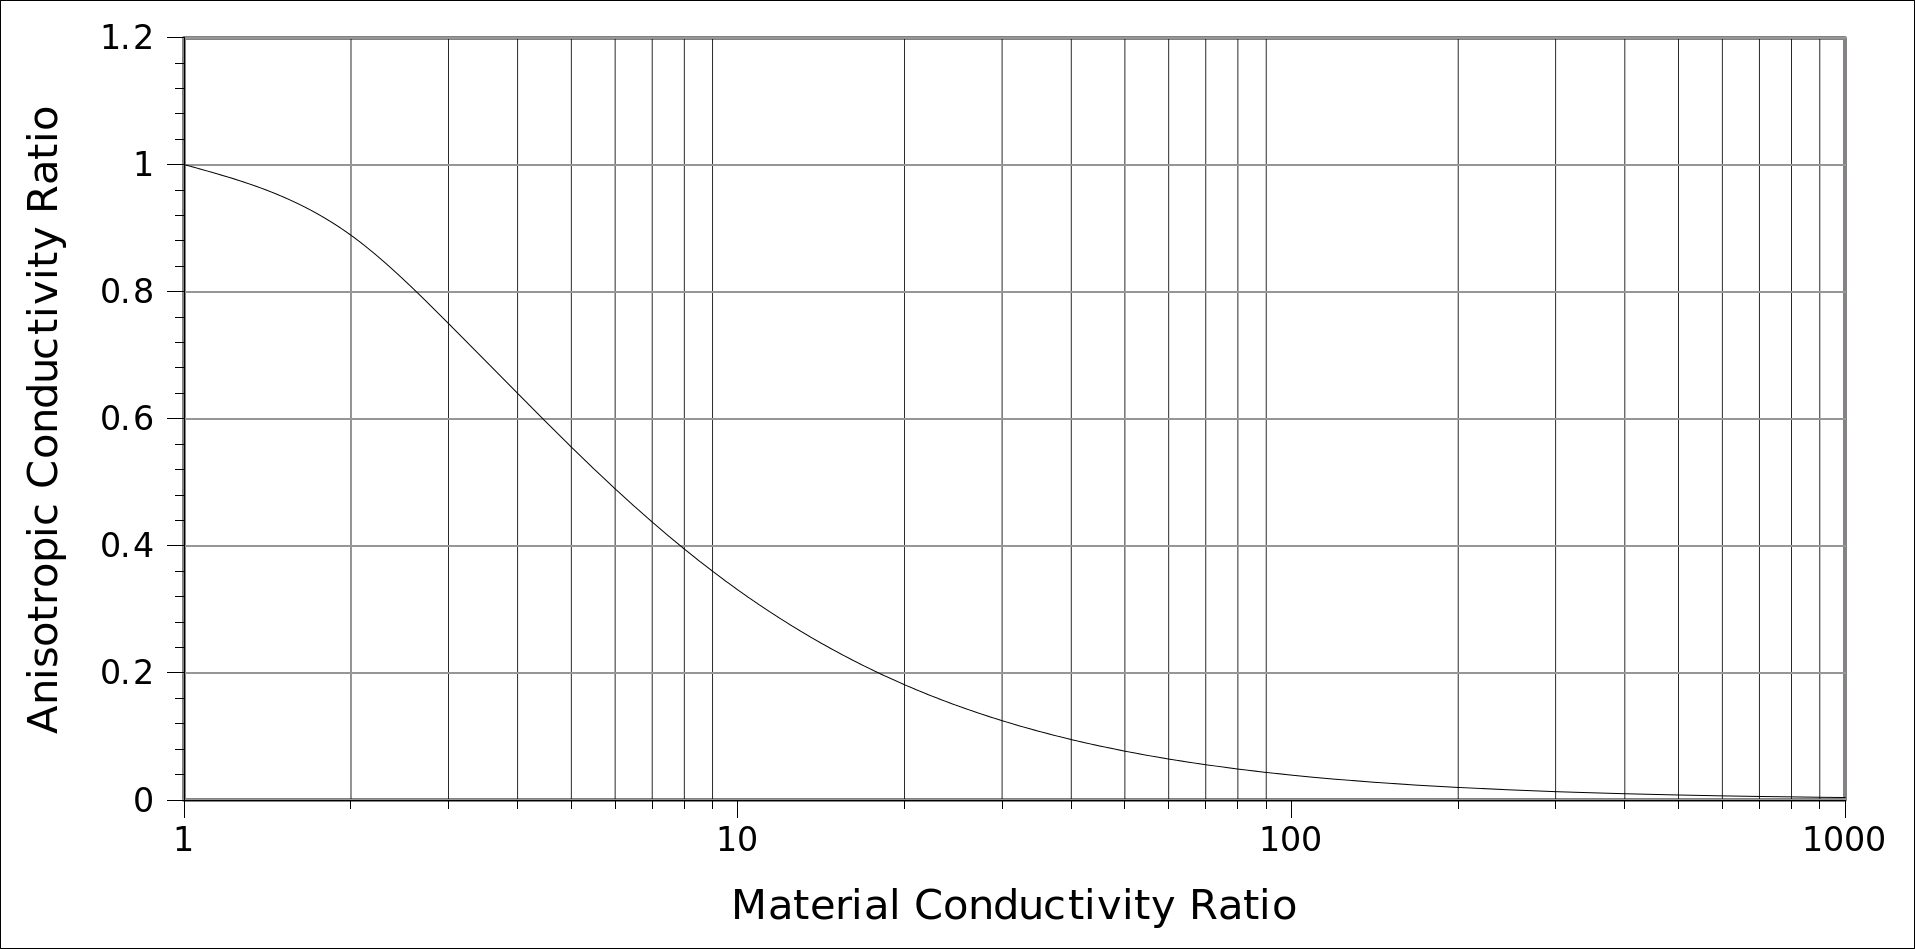
\includegraphics[width=0.7\textwidth]{fig/anisovmaterial_ratios.png}
\label{fig:anisovmatl_rats}
\caption{Anisotropic Conductivity Ratio vs. Material Conductivity Ratio for the
layered geometry used in the benchtop experiments. It may take a very large
material conductivity ratio in order to achieve a relatively minor anisotropic
conductivity ratio.}
\end{figure}

\section{Comprehensive Benchtop Measurements}

While enough benchtop measurements were taken to give a vague idea as to the
effectiveness of this measurement technique, there were not nearly enough
measurements to give a statistically valid conclusion regarding the slight
trend we were looking for. In addition to improving the benchtop method, there
need to be many more measurements taken, in order to draw statistically valid
conclusions.

\section{Comprehensive In-Situ Measurements}

The in-situ measurements presented in this document are very limited in scope.
One could easily spend much more time taking more measurements on more snow at
more angles, in order to better quantify the degrees of anisotropy in natural
snowpacks.

\section{A Better Measurement Apparatus}

The current measurement apparatus works. However, it may be difficult to work
with, and does not record insertion angle. An ideal instrument would be easier
to work with, would record this metadata, and do more to keep test data
separated. It is likely that this would make a better project for someone with a
background in electrical engineering instead of a background in a mechanical
engineering, due to the programming and wiring requirements of creating such an
instrument.

\section{Statistical Analyses of Rigor}

Moreover, more rigorous statistical analyses should be applied to the data. The
author has applied relatively elementary analyses to his data.
There are, however, multiple approaches which may be used to quantify the
confidence of a curve showing anisotropy.

\section{Exploration of the Cooling Curve}

In the numerical and analytical models, the cooling curve is all but ignored. It
is believed that cooling curve models will yield analogous results, but this has
not been tested. Because of the importance of cooling curve measurements in the
real world (as they effectively double the number of measurements in a sample),
verification of these expectations of analogous behavior should occur.

\section{A Method for Determining Anisotropic Thermal Conductivity From Measurements}

While this document lays the groundwork for determining anisotropic thermal
conductivity from measurements, a reliable method for converting measurements
into anisotropic thermal conductivities has not been found. Were the data
more reliable and less variable, one may be able to find the portion of the
prediction curve(s) that best fit the data, but based on current measurements,
this doesn't seem likely.

One possibility is that, instead of focusing on the measured conductivities as a
function of angle, that one should focus on the \emph{change} in measured
conductivities with respect to angle. In fact, given low enough degrees of
anisotropy, it may be sufficient to compare linearizations of these curves. Only
with more research can this conjecture be shown to be valid.
